\documentclass[10pt,a4paper]{article}
\usepackage{amsmath,graphicx,subfigure, hyperref, url}

\title{{Master Thesis\\[0.5em]}
       {\bf \huge Development of a game for hand- and eye coordination in children rehabilitation.\\[0.5em]}
       {\bf Weekly Report 7 \& 8}}
\author{Anna Maria Walach, S121540}
\setlength{\parindent}{0mm}
\setlength{\parskip}{\medskipamount}

\begin{document}

\maketitle

\section*{What has been done this week}
In last two weeks:
\begin{itemize}
\item I've had a conversation with the occupational therapist, whom explained to me what a coordination game should look like, what the game properties should be and told me about examples of game she use in such cases with her patients. 
\item I prepared a list of items that I want to test
\item I made extensive research to gather "theoretical" properties of all the devices
\item I started testing of the devices in the area of "detailed gesture recognition"
\end{itemize}
\begin{figure}
\centering
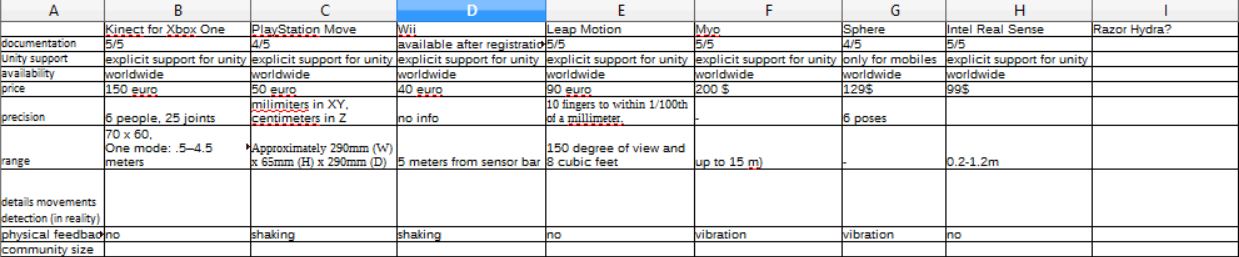
\includegraphics[scale=0.4]{comparison.png} 
\caption{The list of tested devices, updated list of criteria and current results of analysis.}
\end{figure}

\section*{Project status according to the study plan}
%all nice and well
I should have been done with testing by the end this week, which I'm not, but because I already started the implementation part, it is acceptable delay. 

\section*{Plan for the next weeks}
In next week I want to finish the testing and decide on application test days and the devices to be used. 
In next weeks I want to fully commit to development of the game. 
\bibliography{../thesis/bibliography/Bibliography}


\end{document}
